\documentclass[dutch,a4paper,10pt]{report}

\usepackage[default]{droidserif}
\usepackage{inconsolata}
\usepackage[T1]{fontenc}
\usepackage[utf8]{inputenc}
\usepackage[english,dutch]{babel}
\usepackage[chapter]{minted}
\usepackage{a4wide}
\usepackage[font=small,format=plain,labelfont=bf,up,textfont=it,up]{caption}
\usepackage{xcolor}
\usepackage{graphicx}
\usepackage[pdftex]{hyperref}
\usepackage[inline]{enumitem}
\usepackage{amsmath}
\usepackage{units}
\usepackage{xspace}
\usepackage[toc,page]{appendix}

\usepackage{tikz}
\usetikzlibrary{trees}
\usetikzlibrary{decorations}
\usetikzlibrary{arrows,positioning,shapes}
\usetikzlibrary{calc}
\usetikzlibrary{decorations.markings}
\usetikzlibrary{automata}

% Custom commands
\newcommand{\autonerf}{\textsc{Autonerf}\xspace}
\renewcommand{\appendixname}{Bijlage}
\renewcommand{\appendixtocname}{Bijlagen}
\renewcommand{\appendixpagename}{Bijlagen}

\begin{document}
    \begin{titlepage}

\Huge \textsc{\bfseries \autonerf} \normalsize \\

\vfill

\begin{minipage}[b][1em][b]{\linewidth}
    Hogeschool van Arnhem en Nijmegen, Ruitenberglaan 26 te Arnhem
\end{minipage}

\begin{minipage}[b][2em][b]{\linewidth}
\end{minipage}

\begin{minipage}[b][4em][b]{\linewidth}
    \begin{tabular}{l l }
        Projectgroep: & Ramon Kleiss \texttt{<ramonkleiss@gmail.com>} \\
        & Niek van der Straaten \texttt{<niekvds@gmail.com>} \\
        \\
        Begeleider: & Hugo Arends \texttt{<hugo.arends@han.nl>} \\
    \end{tabular}
\end{minipage}

\end{titlepage}

    \tableofcontents
    \chapter{Inleiding}
\label{chap:introduction}

% Waar gaat het verslag over, wat zijn de achtergronden van het project
% (in het kort)?
%
% Hoe is de logische opbouw van het verslag?

Dit verslag is geschreven in opdracht van de Hogeschool van Arnhem en Nijmegen
in het kader van de minor Embedded Vision Design (EVD) aan de opleiding Embedded
Systems Engineering (ESE). Het beschrijft hoe het project van de studenten is
ontwikkeld en waarom bepaalde ontwerp keuzes zijn gemaakt gedurende de
ontwikkeling van het product.

Het doel van het project was om een autonome \emph{Nerfgun} (zie figuur
\ref{fig:nerfgun}) te ontwikkelen. Dit product moet in staat zijn om een
\emph{marker} te herkennen en daar vervolgens een \emph{nerfdart} (figuur
\ref{fig:nerfdart}) op af te vuren. De officiele projectomschrijving was als volgt:

\begin{quotation}
\emph{Uiterlijk week 20 van het academisch jaar 2013-2014 zal een systeem
ontwikkeld zijn die autonoom een Nerf-gun kan afvuren op bewegende, gemarkeerde,
doelwitten. Het systeem moet gebruik maken van camera beelden om deze doelwitten
te vinden binnen een omgeving.}
\end{quotation}

Het systeem is gedoopt tot \bold{\autonerf}, een samenvoeging van \emph{autonoom}
en \emph{Nerf}. In dit verslag worden de resultaten van de verschillende
projectfasen besproken en nader toegelicht.

Het eerste deel dat zal worden beschreven is het functioneel ontwerp (hoofdstuk
\ref{chap:functional}). Hier zal functioneel beschreven worden wat het systeem
moet doen. Er zal verder niet worden ingegaan op hoe het systeem dit bereikt.
Het hoofdstuk Technische Specificatie (hoofdstuk \ref{chap:technical}) zal hier
verder op ingaan. Hoofdstuk \ref{chap:realisation} zal de realisatie van het
project beschrijven. Er zal besproken worden welke beslissingen er gemaakt zijn
en waarom deze gemaakt zijn. Uiteindelijk zullen de resultaten van het testen
(hoofdstuk \ref{chap:testing}) besproken worden. Daarnaast zal in hoofdstuk
\ref{chap:conclusion} een conclusie worden getrokken en zullen eventuele
aanbevelingen worden gedaan voor het verdere ontwikkeling van het product.

    \chapter{Functioneel Ontwerp}

% systeembeschrijving op het hoogste niveau; wat moet het systeem doen,
% niet hoe; hoe ziet de gebruiker het systeem; systeem opdelen in
% functionele blokken en definiëren van de interfaces daartussen

    \chapter{Technisch Ontwerp}

% architectuur van de gekozen oplossing (blokschema's, hiërarchische schema's,
% architectuurschema's, wat in hardware, wat in software); afwegen van
% alternatieven; globale oplossing van de belangrijkste of meest complexe
% deelfuncties en onderdelen, toestandsdiagrammen van (belangrijkste of meest
% complexe) functies, gekozen implementatie van datastructuren, eventueel
% pseudo-code; hoe worden de functies en onderdelen gerealiseerd

\section{Hardware}
\label{sec:hardware}

\subsection{Opzet}
\label{sub:opzet}
Het initiële ontwerp was een combinatie systeem van FPGA en een CPU. Door in 
de FPGA operatoren te implementeren moest er een hoge frame-rate gehaald kunnen 
worden. Mede door de communicatie complexiteit is er afgezien van een FPGA 
systeem en is er gekozen voor een snelle processor met Linux. Zo kan er gemakkelijk 
gebruik worden gemaakt van een USB camera.

\subsection{Ontwikkelingsbord}
\label{sub:devboard}
De markt voor Linux gebaseerde ontwikkelingsbordjes is redelijk uitgebreid. Voor 
dit project zijn er echter een aantal eisen.

\begin{itemize}
	\item 2 PWM uitgangen t.b.v. de pan en tilt servo's
	\item minimaal 11 GPIO uitgangen t.b.v. 10 darts + veiligheid
	\item zo hoog mogelijke kloksnelheid t.b.v. frame-processing
	\item genoeg geheugen voor minimaal 2 640*480 RGB frames
	\item een community t.b.v. resources
	\item het moet betaalbaar blijven
\end{itemize}

Gezien het erg belangrijk is om voldoende informatie te kunnen vinden over aansturing 
van onder andere hardware en PWM pinnen is er besloten om een BeagleBone Black te 
nemen. Met 6 PWM kanalen, 69 GPIO's, 512Mb DDR3 RAM en een 1GHz CPU is dit een prima 
apparaat om te gebruiken voor dit project.

\subsection{Cape}
\label{sub:cape}
Om de veiligheid van personen om het systeem te kunnen garanderen wordt er wederom 
gebruik gemaakt van een hardware-matig beveiligingssysteem. Bestaand uit een 
vereenvoudigde versie van de PC + Arduino combinatie.
De interface zal bestaan uit een 3-tal LEDs en een 2-tal knoppen. De 3 LEDs zullen 
de gebruiker laten weten of dat de applicatie aan staat of niet, of dat het apparaat 
kan schieten of niet en of dat er herladen moet worden.
Met de 2 knoppen kan het schieten en draaien hardware-matig geactiveerd en gedeactiveerd 
worden. Daarnaast zit er een knop op om aan te geven dat het systeem herladen is.
De interface dient als cape op de BeagleBone Black gemonteerd te worden. Verder zal de 
cape de nodige voedingsspanningen voorzien aan de kleppen, servo's en de BeagleBone Black 
zelf. Door de applicatie automatisch te laten starten op de BeagleBone Black is het doel 
een plug-and-play systeem te maken.
    \chapter{Realisatie}

% detailontwerp met bijbehorende berekeningen (voedingsstromen, waarden van
% componenten); aansluitschema's van kabels en connectors; detailschema’s van
% de hardware en listings van de software worden in de bijlagen opgenomen

    \chapter{Testen en Resultaten}
\label{chap:testing}

% korte ondubbelzinnige weergave hoe de hardware en software getest is; tests
% per module, integratietest; wat is de testopzet geweest en wat zijn de
% uiteindelijke resultaten; voldoet het aan de gestelde eisen; duidelijk
% omschrijven welke eventuele problemen er nog zijn en hoe deze mogelijk zijn
% te verklaren; eventuele 'work arounds', aanbevelingen; de testen moeten
% zodanig omschreven zijn dat elke test door anderen te reproduceren is

De software en hardware is in verschillende onderdelen getest.
\begin{itemize}
	\item GPIO en servo test;
	\item Camera acquisitie test + benchmark;
	\item Frame processing test.
\end{itemize}

\section{GPIO en servo}
\label{sec:gpioTest}

\subsection{Software}
\label{sub:gpioSoft}
Op basis van een aantal tutorials is er test code geschreven om een GPIO te
testen. Met een multimeter kan er gecontrolleerd worden of de GPIO correct
geconfigureerd is. Daarnaast kan er met een draadje een knopje gesimuleerd
worden.

De GPIO's waren redelijk snel werkend mede dankzij de duidelijke tutorials
beschikbaar voor de BeagleBone Black.

De servo's worden via hardware PWM aangestuurd. Met dank aan wat informatie
op het internet en de GPIO tutorials was de PWM zo aan de praat. Middels een
simpele transistor schakeling is er een servo aan een hardware PWM pin te koppelen.
Door eerst een LED te laten dimmen kan de PWM functie gevalideerd worden.
Vervolgens wordt er een servo aan gekoppelt om de PWM frequentie en puls breedte
te bepalen.

Na de tests is er test software geschreven voor alle hardware aansturingen
zodat er via de command line de interface getest kon worden.

\subsection{Hardware}
\label{sub:gpioHard}

De hardware is eerst op een bench getest om eventuele schade als gevollig van
een foutief ontwerp aan de BeagleBone Black te voorkomen. Alle pinnen zijn
nagemeten voor eventuele kortsluitingen. Daarnaast is de flip-flop schakeling
los van de rest van het systeem getest.

Na een test bleek de flip-flop schakeling niet helemaal te werken. Dit is opgelost
door een RC schakeling tussen de /Q output en D input. Daarna bleken de MOSFETs
ook niet helemaal correct te werken. Het bleek dat de MOSFETs niet voldoende
inschakelen bij 3,3V maar pas vanaf 5V voldoende stroom door laten. Dit probleem
is eenvoudig opgelost middels een 5V pull-up weerstand en een 2,4V zener diode 
(zie bijlage \ref{app:sig-conv-schematic} en \ref{app:sig-conv-pcb}).

\section{Camera acquisitie}
\label{sec:camAcq}

De camera acquisitie is geschreven op basis van een tutorial voor video for
linux. Gezien de acquisitie met voldoede snelheid moet gebeuren is er een
benchmark uitgevoerd op de code. Met een frame-rate van 10 - 30fps is er
geconcludeerd dat de acquisitie voldoende snelheid heeft om een prima
systeem te bouwen.

\section{Frame processing}
\label{sec:framePross}

Veel van de operatoren om het frame te verwerken zijn al gemaakt voor het
practicum. Deze zijn dus uitgebreid getest via de QT applicatie en op het
target. Daarnaast is de code voor de BeagleBone Black omgebouwd om een
plaatje in te lezen, het plaatje te verwerken en een plaatje als output
te geven. Dit omdat het systeem van het practicum geen kleuren plaatjes
accepteerd. Op deze manier is het dus wel mogelijk om de RGB filter te
testen.

De resultaten spreken voor zich.

Het originele plaatje.
\begin{figure}
    \begin{center}
        % \includegraphics[scale=0.35]{figures/origineel.png}
    \end{center}
    \caption{Het originele plaatje.}
    \label{fig:org}
\end{figure}

Omdat enkel rode data interessant is.
\begin{figure}
    \begin{center}
        % \includegraphics[scale=0.35]{figures/red_filterd.png}
    \end{center}
    \caption{Het grijswaarde plaatje na de rode filter.}
    \label{fig:redFilter}
\end{figure}

Omdat wel alle data duidelijk moet zijn, rek het contrast uit.
\begin{figure}
    \begin{center}
        % \includegraphics[scale=0.35]{figures/contrast_stretch.png}
    \end{center}
    \caption{Het grijswaarde plaatje na de contrast stretch.}
    \label{fig:contastStretch}
\end{figure}

Enkel echte rode data is interessant, daarom een automatische threshold.
\begin{figure}
    \begin{center}
        % \includegraphics[scale=0.35]{figures/threshold.png}
    \end{center}
    \caption{Het binaire plaatje na de threshold.}
    \label{fig:threshold}
\end{figure}

Blobs aan de randen zijn geen betrouwbare data, vandaar "remove border blobs".
\begin{figure}
    \begin{center}
        % \includegraphics[scale=0.35]{figures/remove_border_blobs.png}
    \end{center}
    \caption{Het binare plaatje na het verwijderen van de blobs aan de randen.}
    \label{fig:removeBorderBlobs}
\end{figure}

Om eventuele schittering op objecten te verwijderen, vul de blob.
\begin{figure}
    \begin{center}
        % \includegraphics[scale=0.35]{figures/fill_holes.png}
    \end{center}
    \caption{Het binaire plaatje na een "fill holes" operatie.}
    \label{fig:fillHoles}
\end{figure}

Label de over gebleven blobs!
\begin{figure}
    \begin{center}
        % \includegraphics[scale=0.35]{figures/label_blobs.png}
    \end{center}
    \caption{Het gelabelde plaatje.}
    \label{fig:labelBlobs}
\end{figure}

Nadat de blob analyzer de grootste blob heeft gevonden wordt het middelpunt doorgegeven.
Dat is in dit geval (xx, yy)pixels.

    \chapter{Conclusie en Aanbevelingen}
\label{chap:conclusion}

% Wat is wel en wat is niet gerealiseerd?
% Wat kan er aan het product worden aangevuld, uitgebreid, verbeterd?



    \begin{appendices}
    \chapter{Initializeren camera met Video4Linux}
\label{app:camera-init}

\begin{minted}{c}
int
camera_open(struct camera_t * camera, const char * device)
{
    size_t                      i;
    struct v4l2_format          format;
    struct v4l2_buffer          buffer;
    struct v4l2_requestbuffers  request;

    if (!camera || camera->fd != -1) {
        return -1;
    }

    // Try to open the camera device
    if ((camera->fd = v4l2_open(device, O_RDWR | O_NONBLOCK)) < 0) {
        LOG_ERROR(strerror(errno));

        return -1;
    }

    // Try to set the camera format
    memset(&format, 0, sizeof(struct v4l2_format));
    format.type                 = V4L2_BUF_TYPE_VIDEO_CAPTURE;
    format.fmt.pix.width        = FRAME_WIDTH;
    format.fmt.pix.height       = FRAME_HEIGHT;
    format.fmt.pix.pixelformat  = V4L2_PIX_FMT_RGB24;
    format.fmt.pix.field        = V4L2_FIELD_INTERLACED;

    if (ioctl(camera->fd, VIDIOC_S_FMT, &format) != 0) {
        LOG_ERROR(strerror(errno));

        return -1;
    }

    if (format.fmt.pix.pixelformat != V4L2_PIX_FMT_RGB24) {
        LOG_CRITICAL("libv4l2 did not accept format RGB24, cannot continue");
        camera_close(camera);

        return -1;
    }

    // Try to request buffers for the camera
    memset(&request, 0, sizeof(struct v4l2_requestbuffers));
    request.count = 2;
    request.type = V4L2_BUF_TYPE_VIDEO_CAPTURE;
    request.memory = V4L2_MEMORY_MMAP;

    if (ioctl(camera->fd, VIDIOC_REQBUFS, &request) < 0) {
        LOG_ERROR(strerror(errno));

        return -1;
    }

    camera->buffers = (struct buffer_t *) calloc(request.count, sizeof(struct buffer_t));

    // Memory map buffers to driver
    for (camera->buffer_count = 0; camera->buffer_count < request.count; camera->buffer_count++) {
        memset(&buffer, 0, sizeof(struct v4l2_buffer));
        buffer.type     = V4L2_BUF_TYPE_VIDEO_CAPTURE;
        buffer.memory   = V4L2_MEMORY_MMAP;
        buffer.index    = camera->buffer_count;

        if (ioctl(camera->fd, VIDIOC_QUERYBUF, &buffer) < 0) {
            LOG_ERROR(strerror(errno));

            return -1;
        }

        camera->buffers[camera->buffer_count].size = buffer.length;
        camera->buffers[camera->buffer_count].data = v4l2_mmap(
            NULL,
            buffer.length,
            PROT_READ | PROT_WRITE,
            MAP_SHARED,
            camera->fd,
            buffer.m.offset
        );

        if (camera->buffers[camera->buffer_count].data == MAP_FAILED) {
            LOG_ERROR(strerror(errno));

            return -1;
        }
    }

    for (i = 0; i < camera->buffer_count; i++) {
        memset(&buffer, 0, sizeof(struct v4l2_buffer));
        buffer.type     = V4L2_BUF_TYPE_VIDEO_CAPTURE;
        buffer.memory   = V4L2_MEMORY_MMAP;
        buffer.index    = i;

        if (ioctl(camera->fd, VIDIOC_QBUF, &buffer) < 0) {
            LOG_ERROR(strerror(errno));

            return -1;
        }
    }

    return 0;
}
\end{minted}

    \chapter{Launcher ontwerp}
\label{app:launcher}

\begin{figure}
    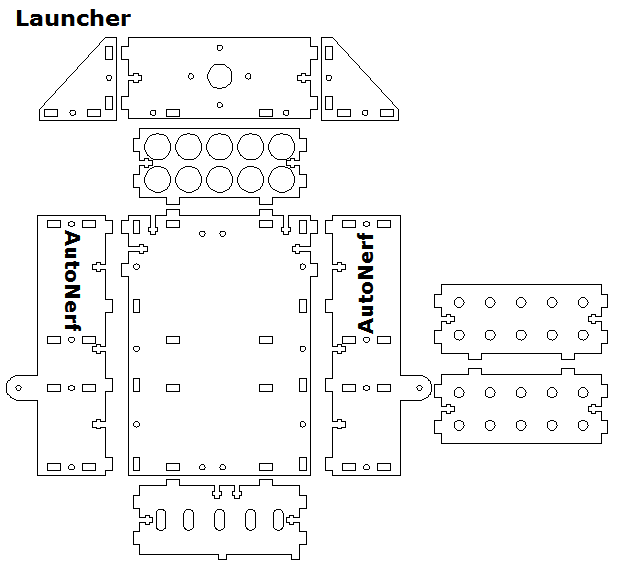
\includegraphics[scale=0.5]{figures/appendix/launcher.png}
    \caption{Ontwerp \emph{launcher}}
\end{figure}

    \chapter{Pan platform ontwerp}
\label{app:pan-platform}

\begin{figure}
    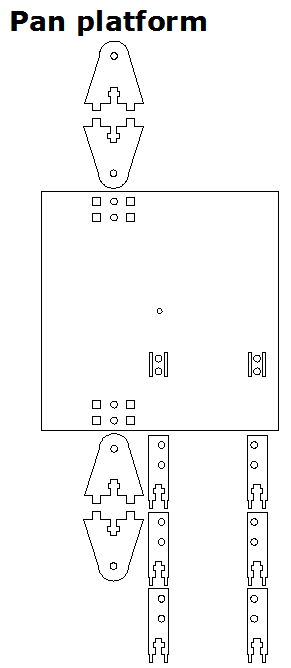
\includegraphics[scale=0.5]{figures/appendix/pan.png}
    \caption{Ontwerp \emph{pan platform}}
\end{figure}

    \chapter{Base platform ontwerp}
\label{app:base-platform}

\begin{figure}
    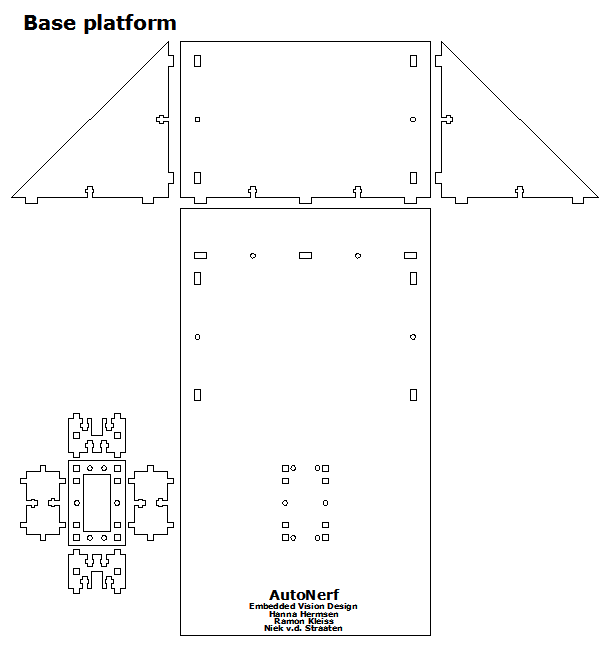
\includegraphics[scale=0.5]{figures/appendix/base.png}
    \caption{Ontwerp \emph{base platform}}
\end{figure}

    \chapter{PCB ontwerpen}
\label{app:pcb}

\begin{figure}
    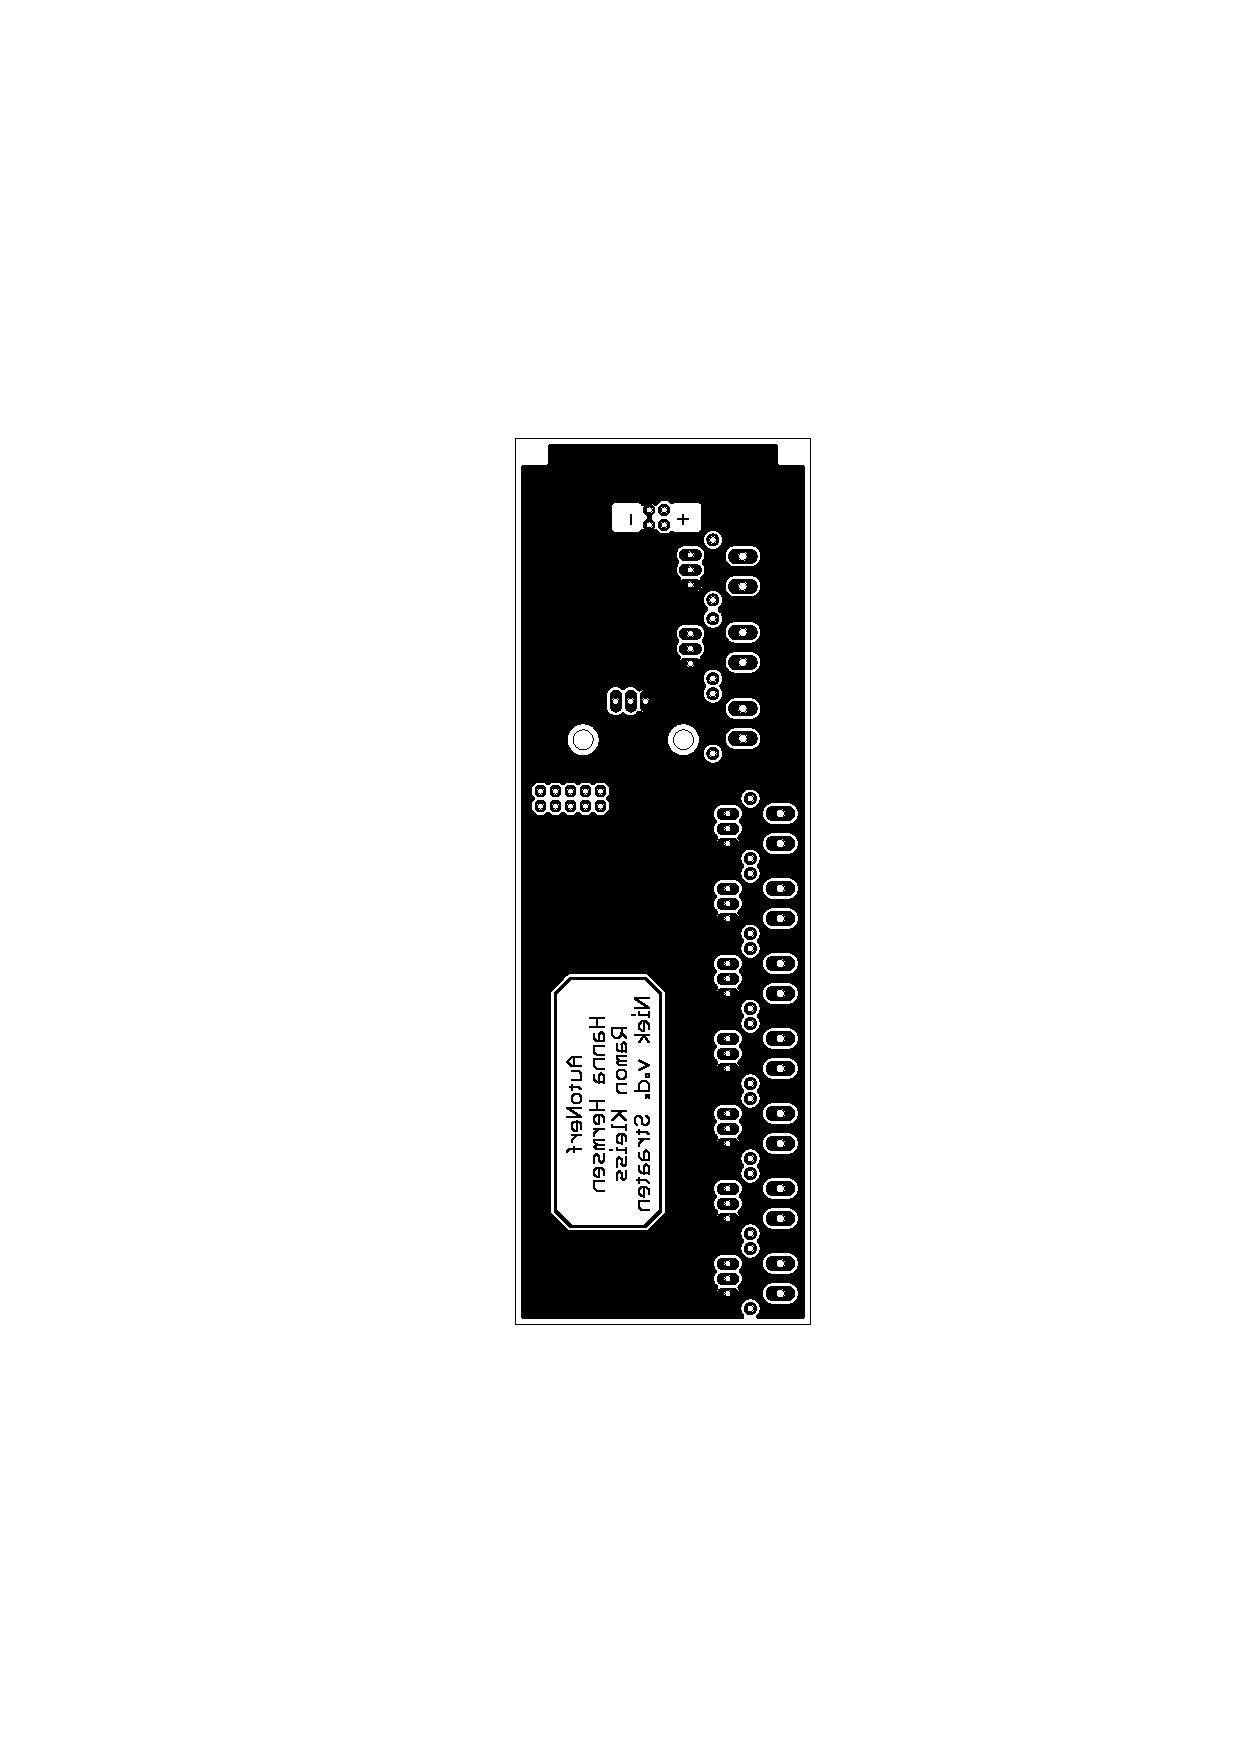
\includegraphics[scale=0.75]{figures/controller_top.pdf}
    \caption{\emph{Controller} ontwerp \emph{top}}
\end{figure}

\begin{figure}
    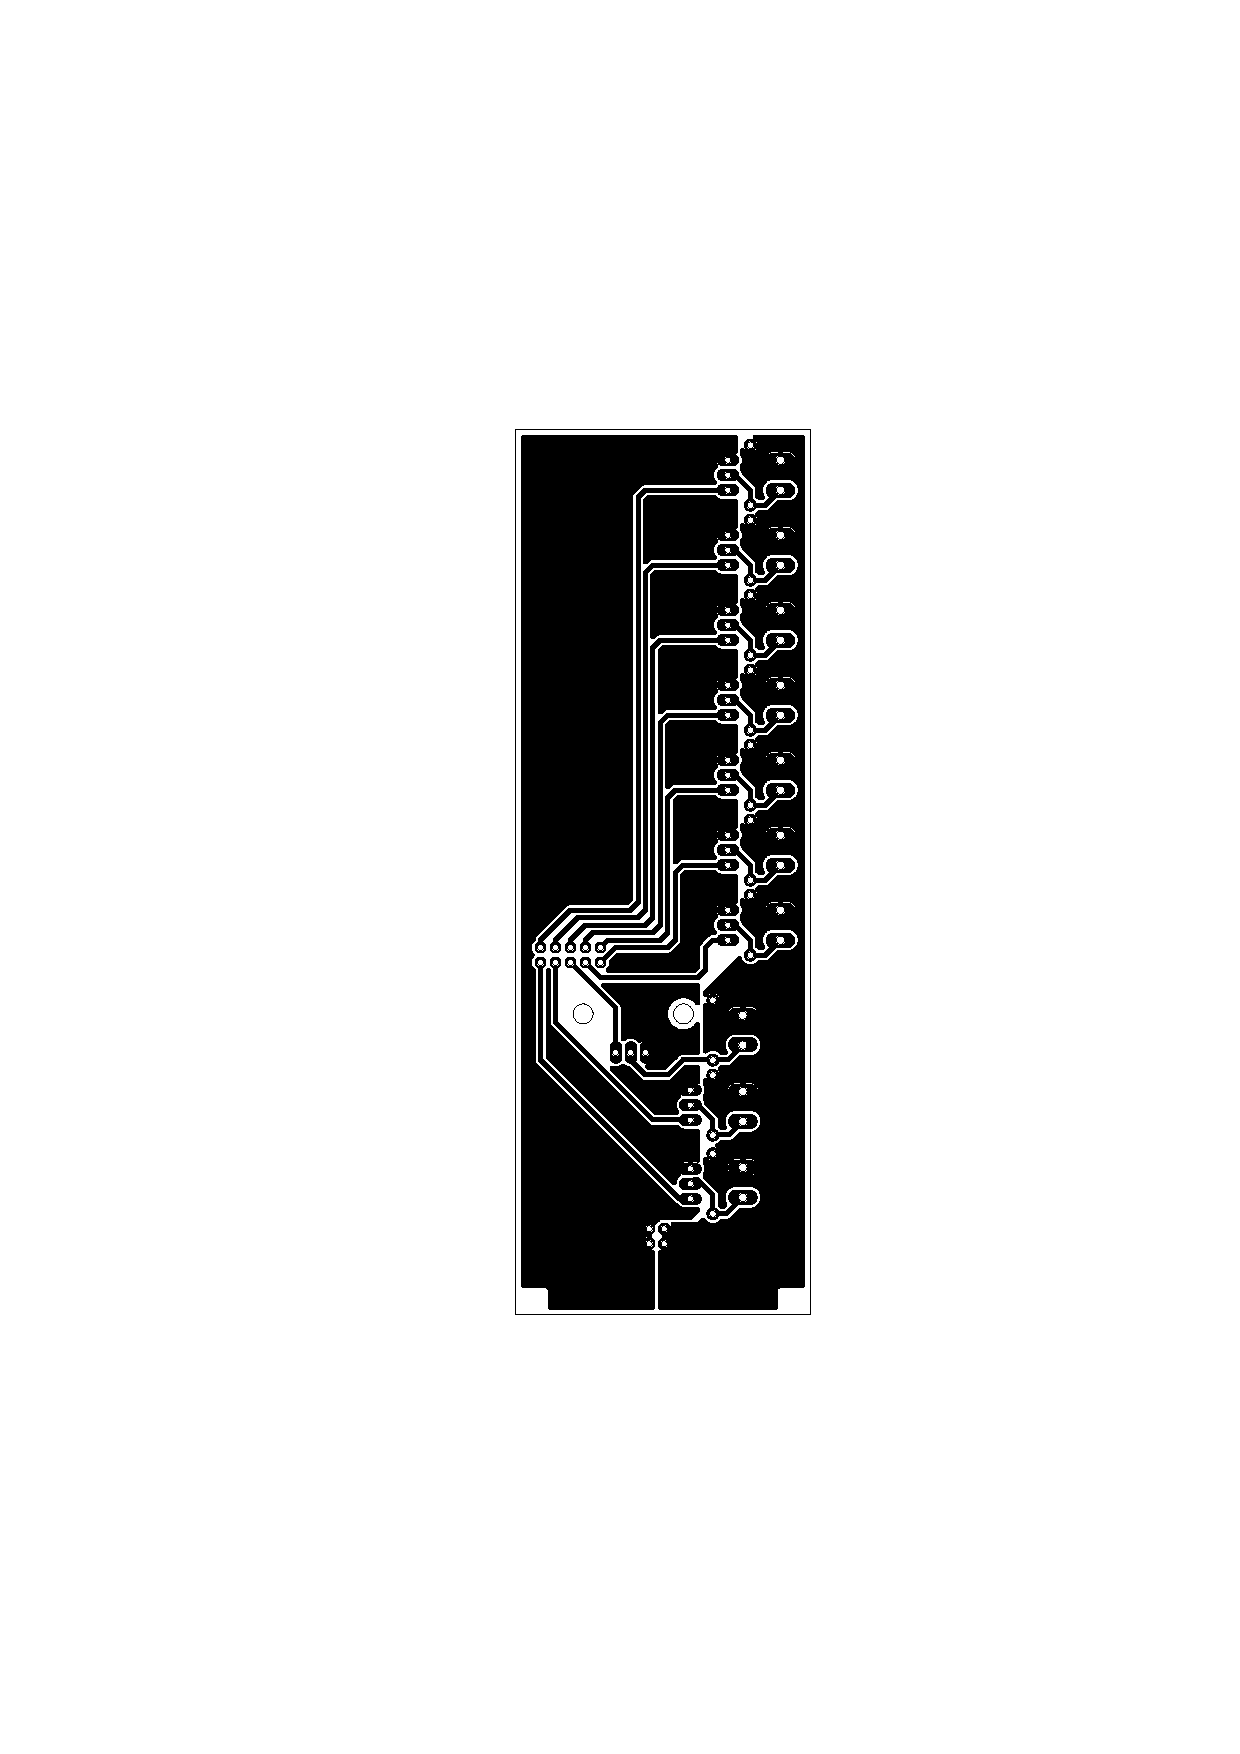
\includegraphics[scale=0.75]{figures/controller_bottom.pdf}
    \caption{\emph{Controller} ontwerp \emph{bottom}}
\end{figure}

\begin{figure}
    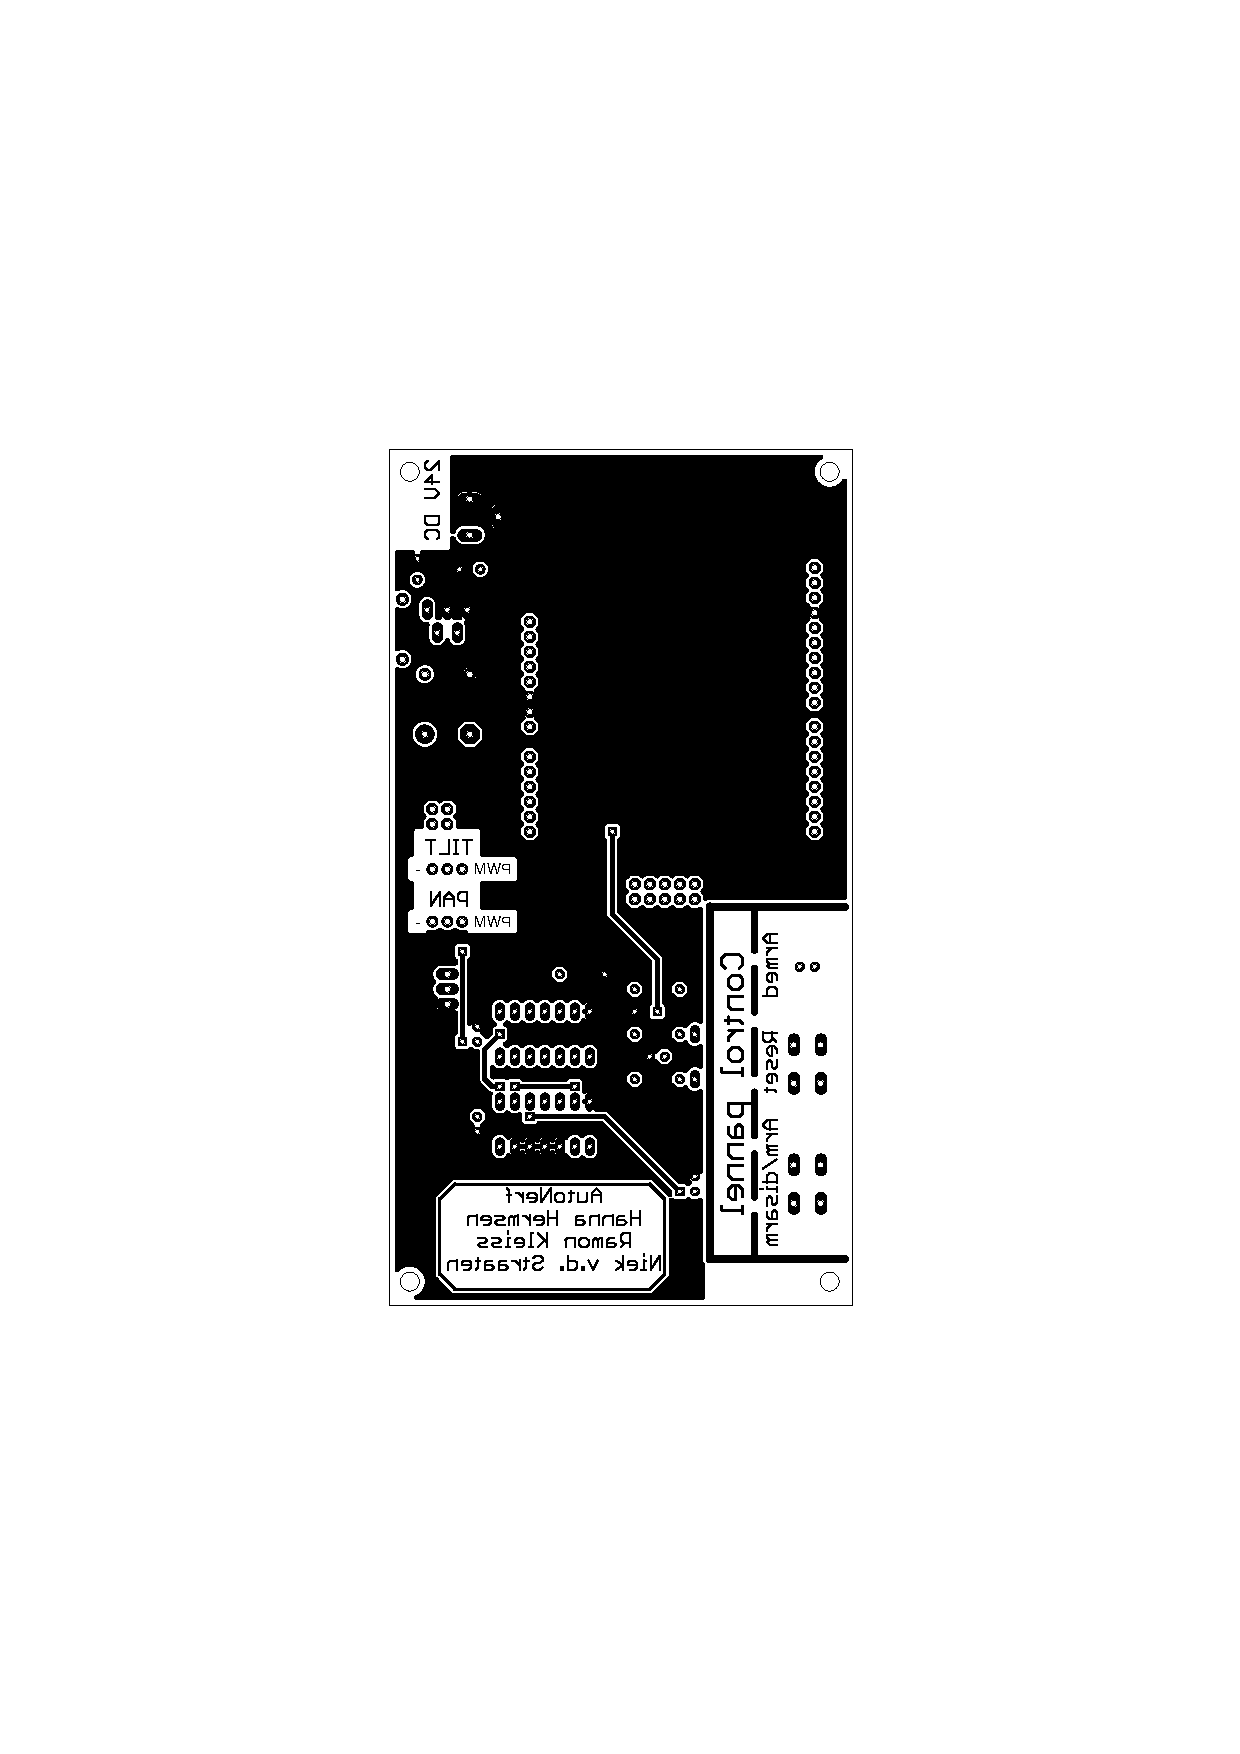
\includegraphics[scale=0.75]{figures/motherboard_top.pdf}
    \caption{\emph{Motherboard} ontwerp \emph{top}}
\end{figure}

\begin{figure}
    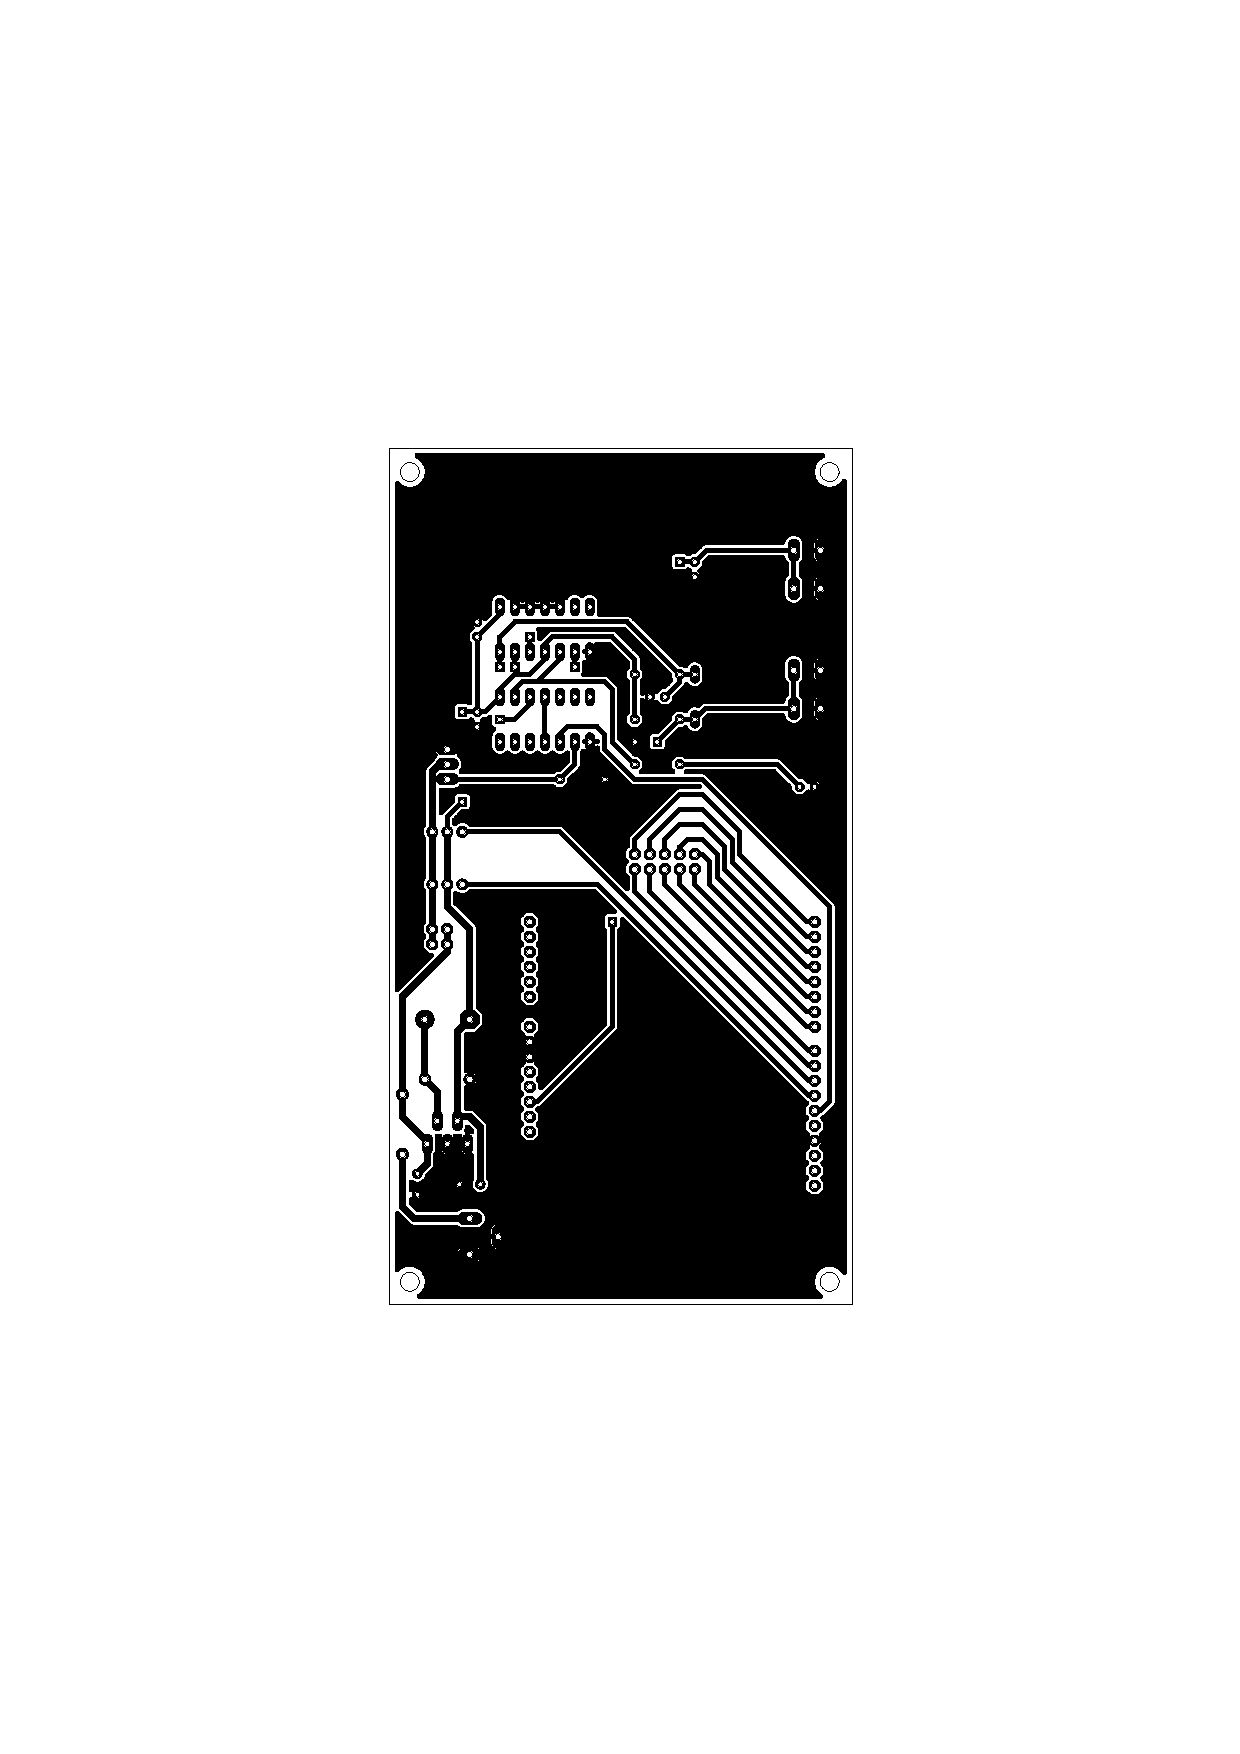
\includegraphics[scale=0.75]{figures/motherboard_bottom.pdf}
    \caption{\emph{Motherboard} ontwerp \emph{bottom}}
\end{figure}

    \chapter{PCB schema's}
\label{app:schematics}

\begin{figure}
    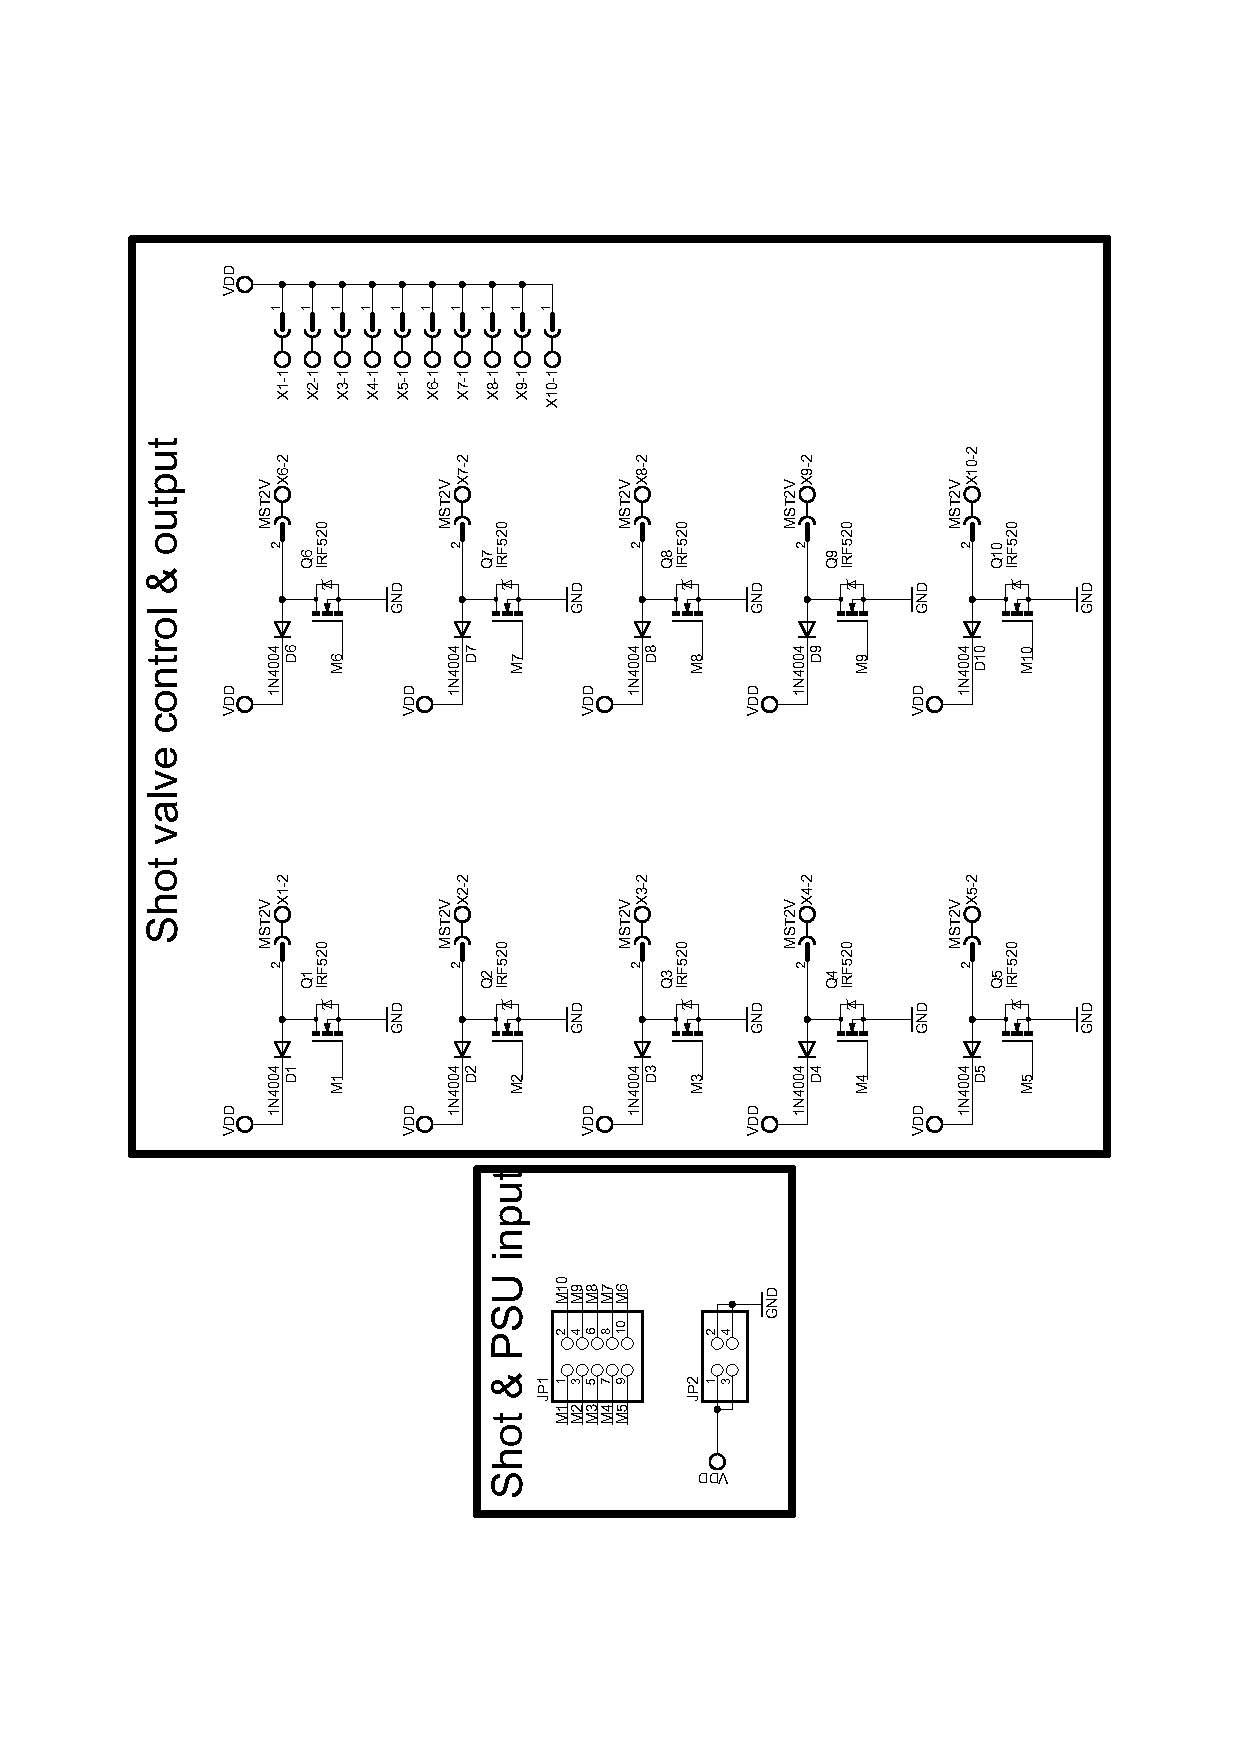
\includegraphics[scale=0.5]{figures/controller_schematic.pdf}
    \caption{Schema van \emph{controller}}
\end{figure}

\begin{figure}
    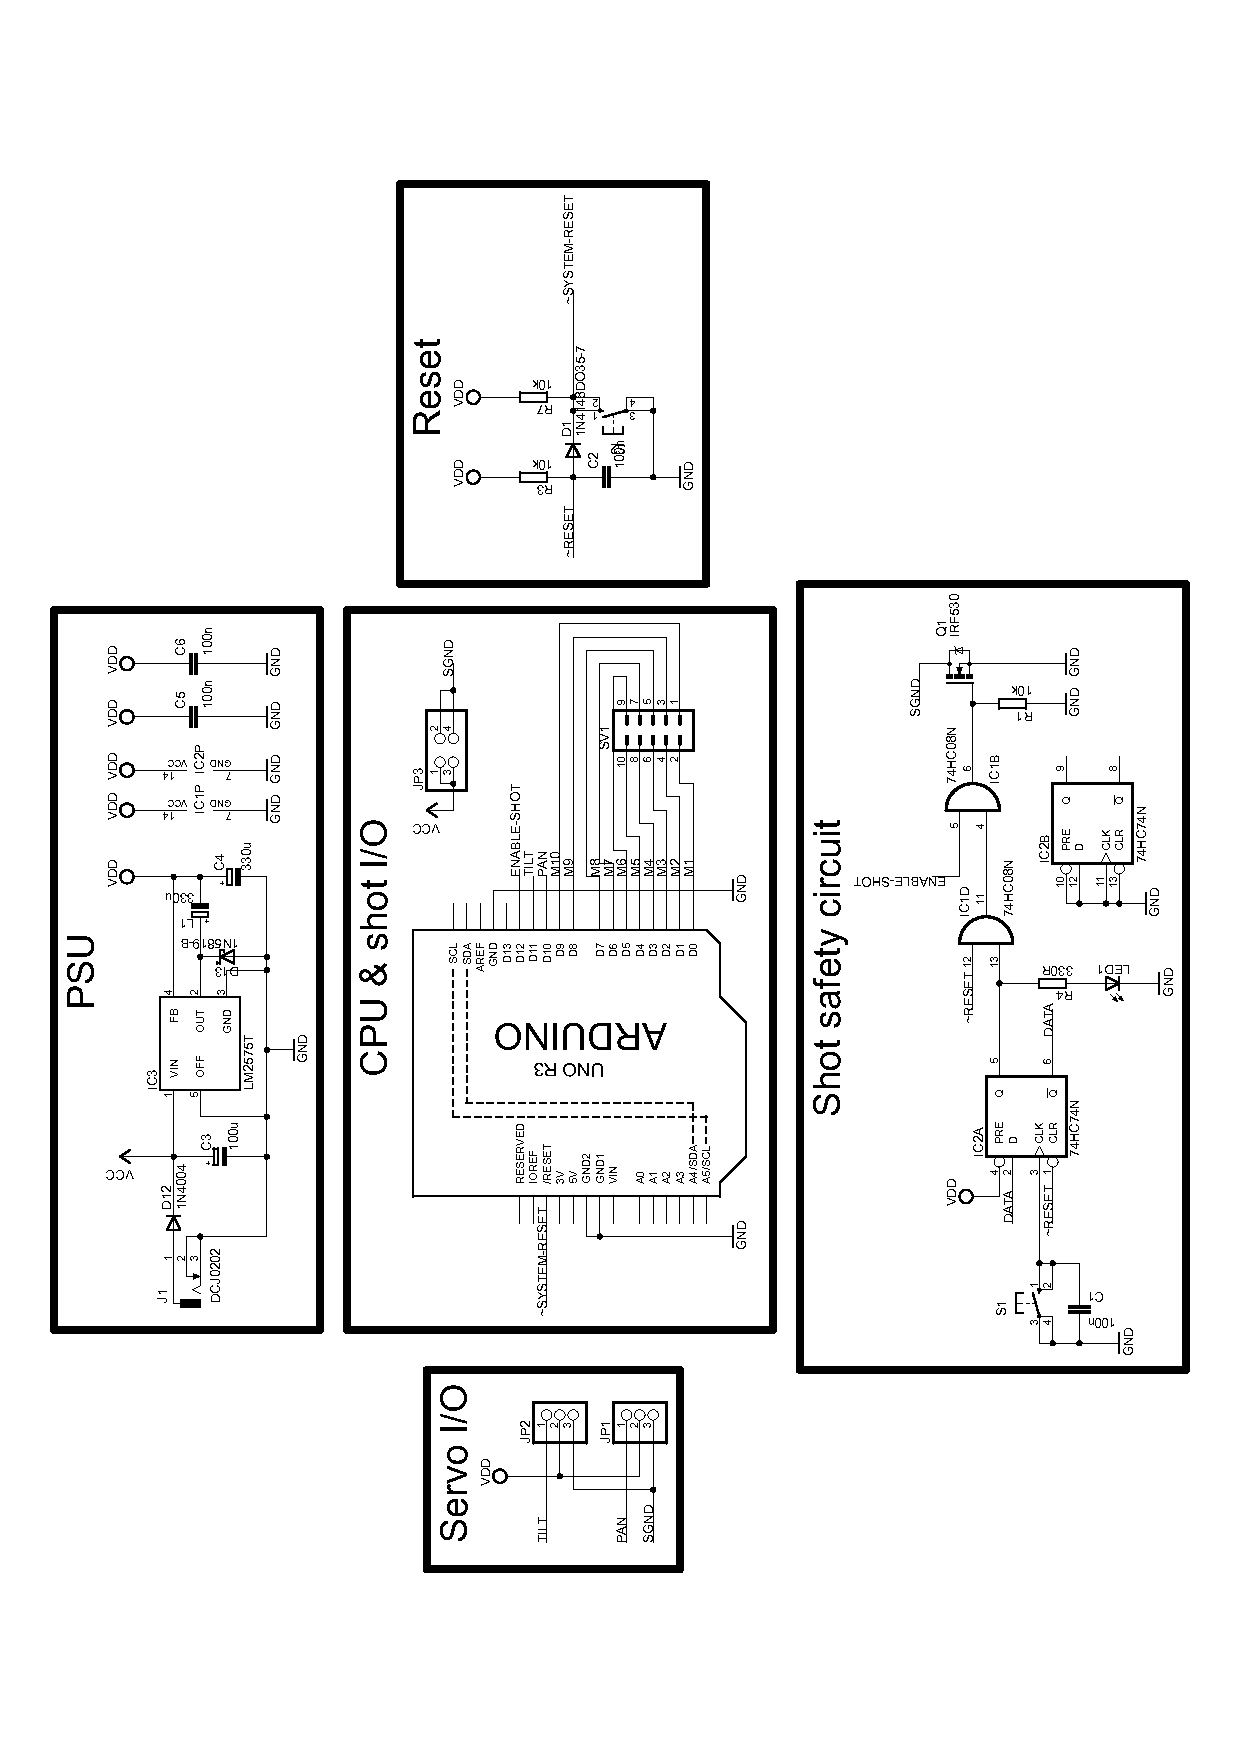
\includegraphics[scale=0.5]{figures/motherboard_schematic.pdf}
    \caption{Schema van \emph{motherboard}}
\end{figure}

    \chapter{Signal Converter Schematic}
\label{app:sig-conv-schematic}

\begin{figure}
    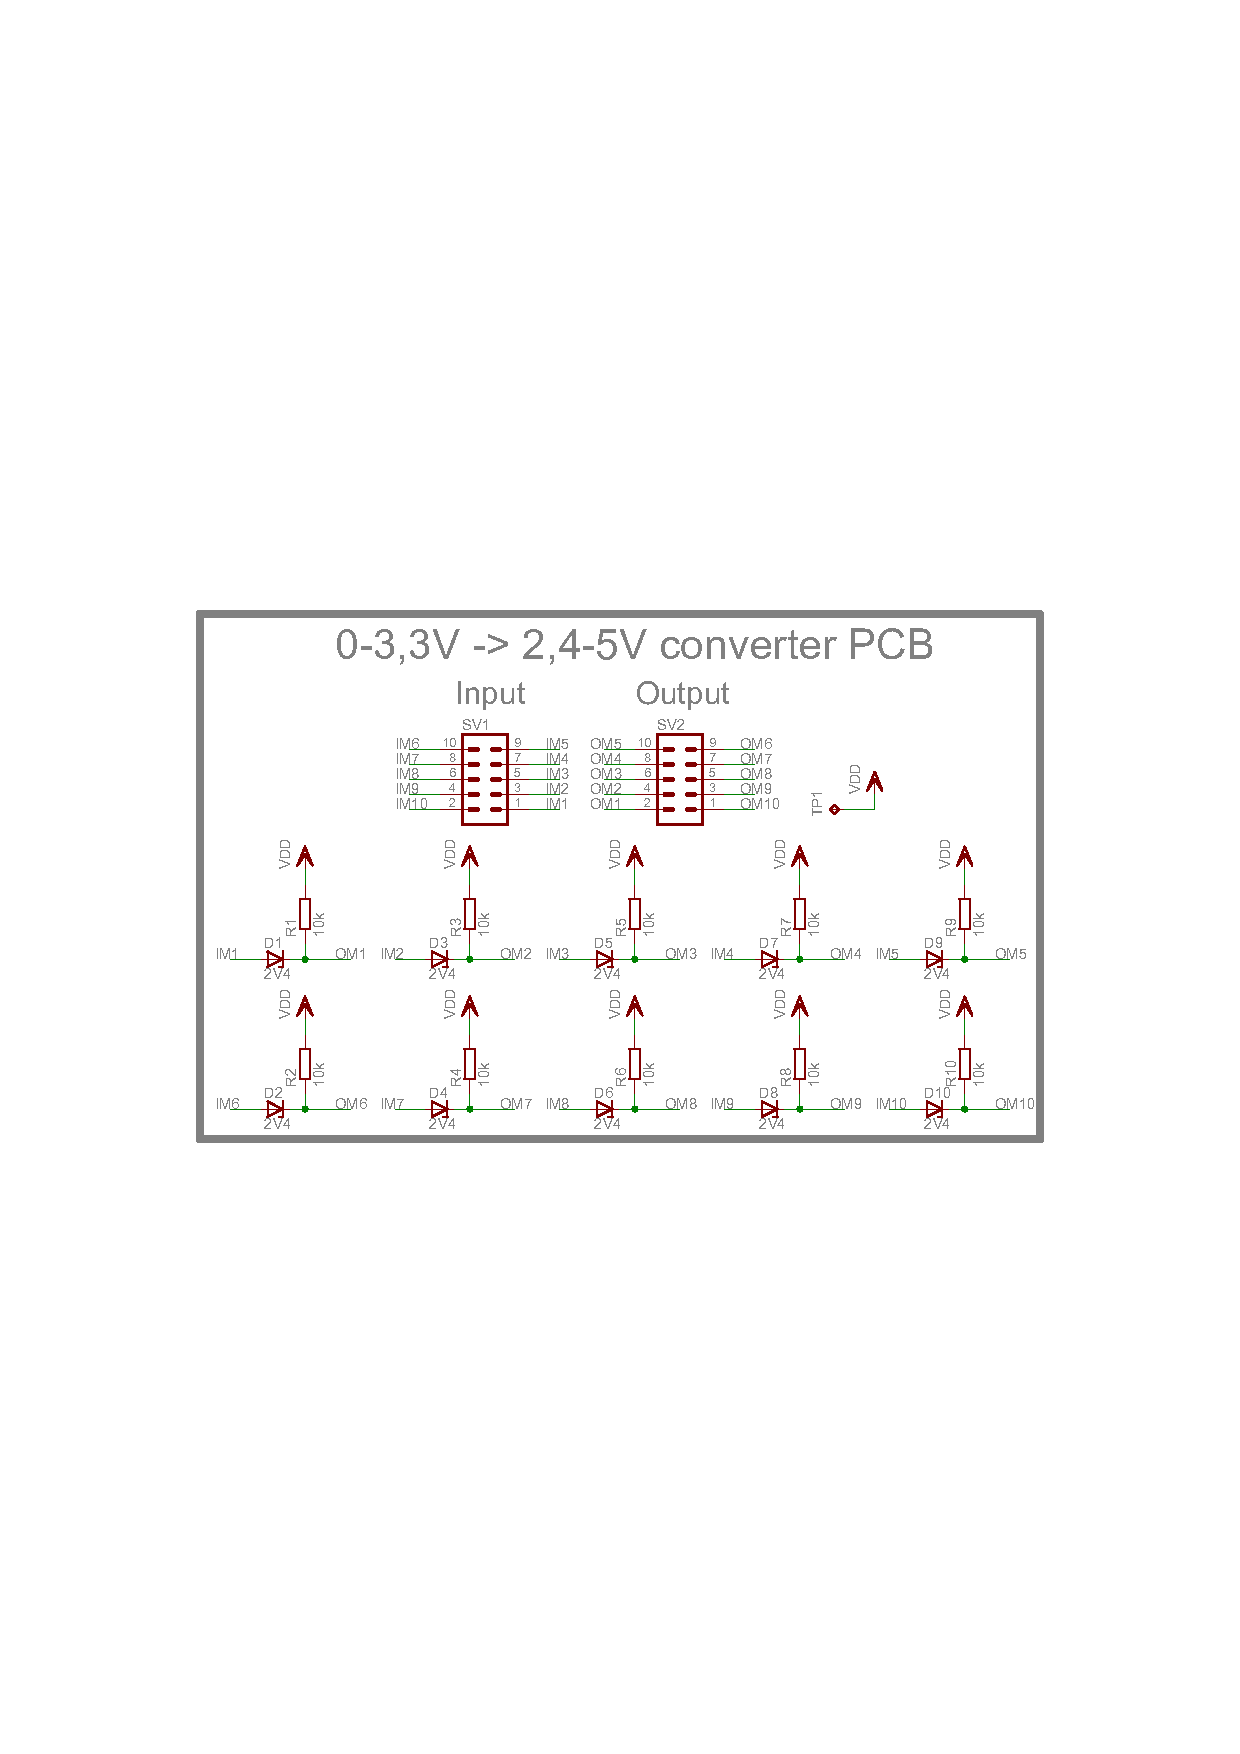
\includegraphics[scale=.75]{appendix/SignaalConverter_schematic.pdf}
    \caption{Schema van \emph{signal converter}}
\end{figure}

\chapter{Signal Converter PCB}
\label{app:sig-conv-pcb}

\begin{figure}
    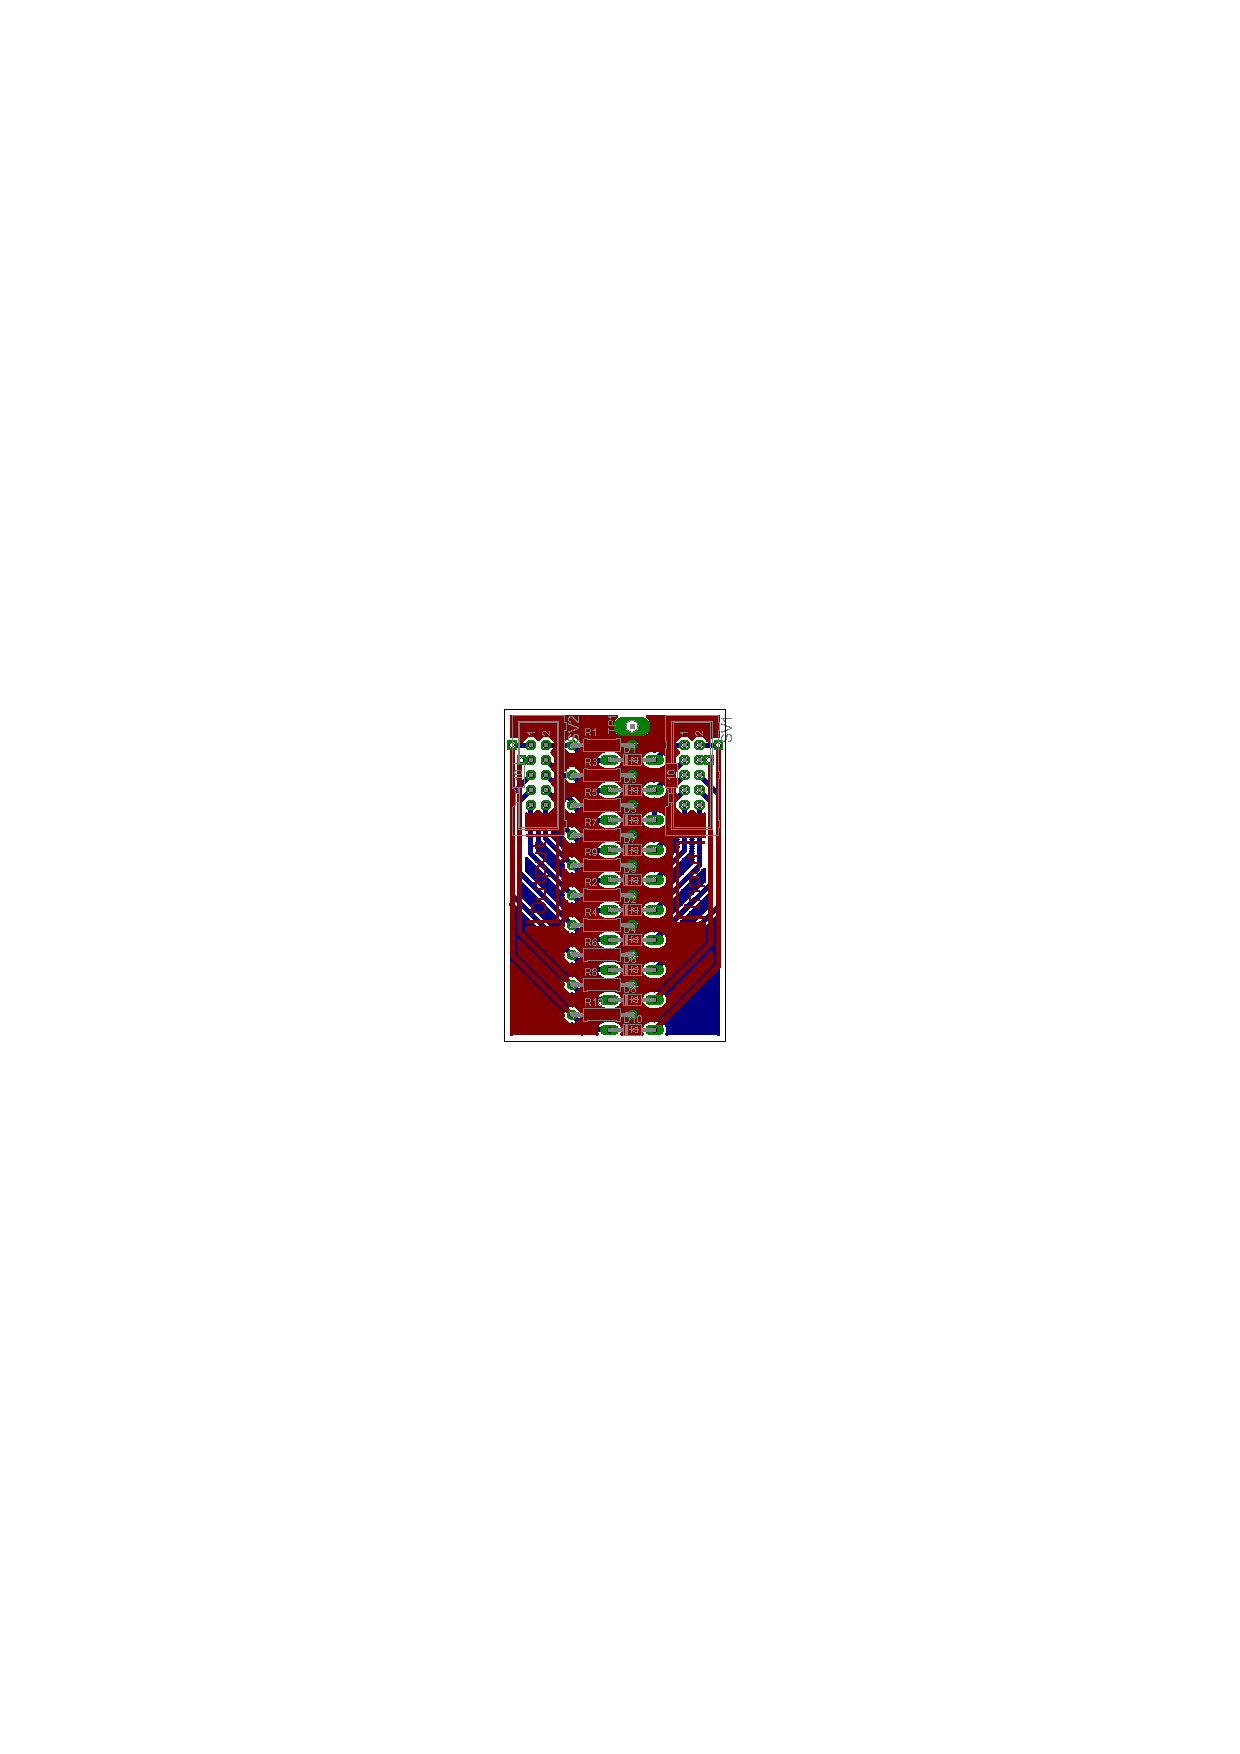
\includegraphics[scale=.75]{appendix/SignaalConverter_pcb.pdf}
    \caption{PCB van \emph{signal converter}}
\end{figure}

    \chapter{BeagleBone Cape Schematic}
\label{app:cape-schematic}

\begin{figure}
    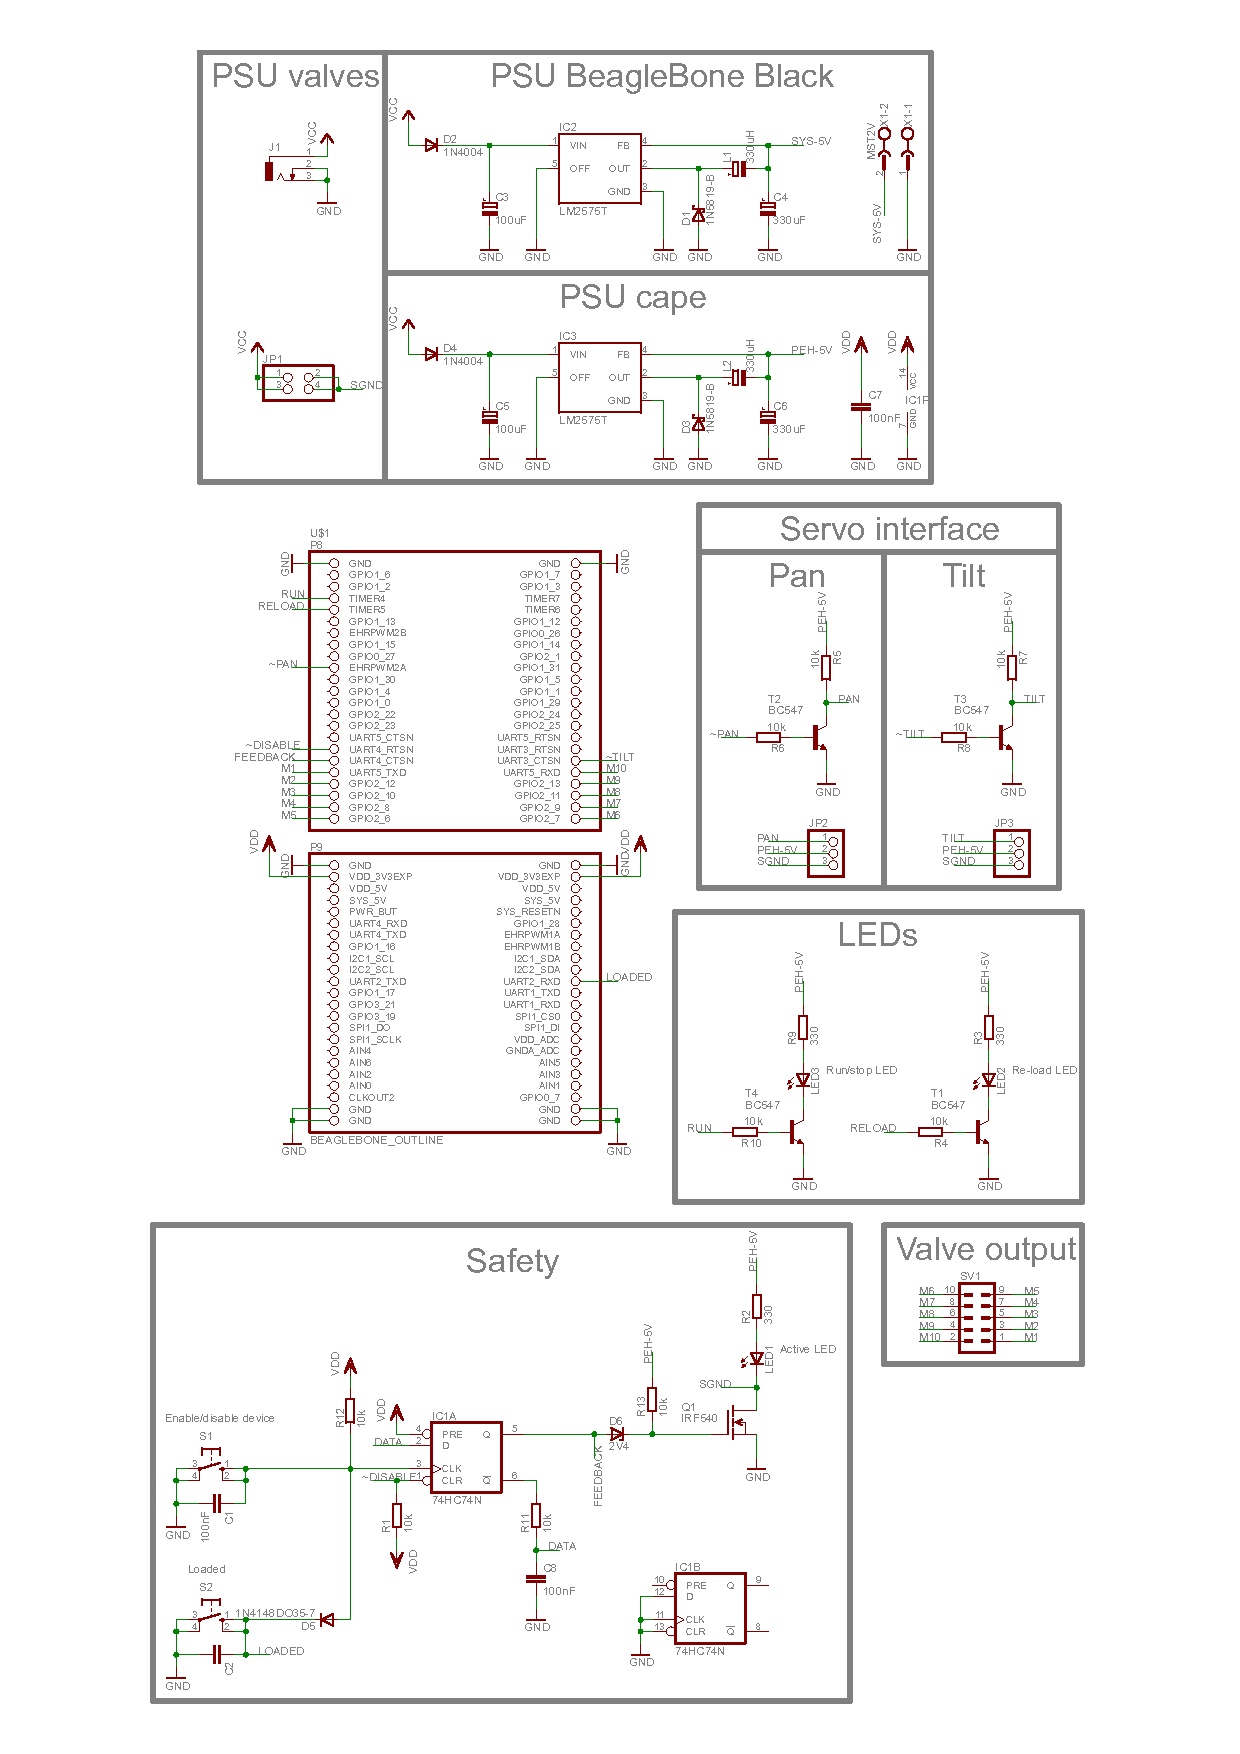
\includegraphics[scale=.75]{appendix/BeagleBoneCape_schematic.pdf}
    \caption{Schema van \emph{BeagleBone cape}}
\end{figure}

\chapter{BeagleBone Cape PCB}
\label{app:cape-pcb}

\begin{figure}
    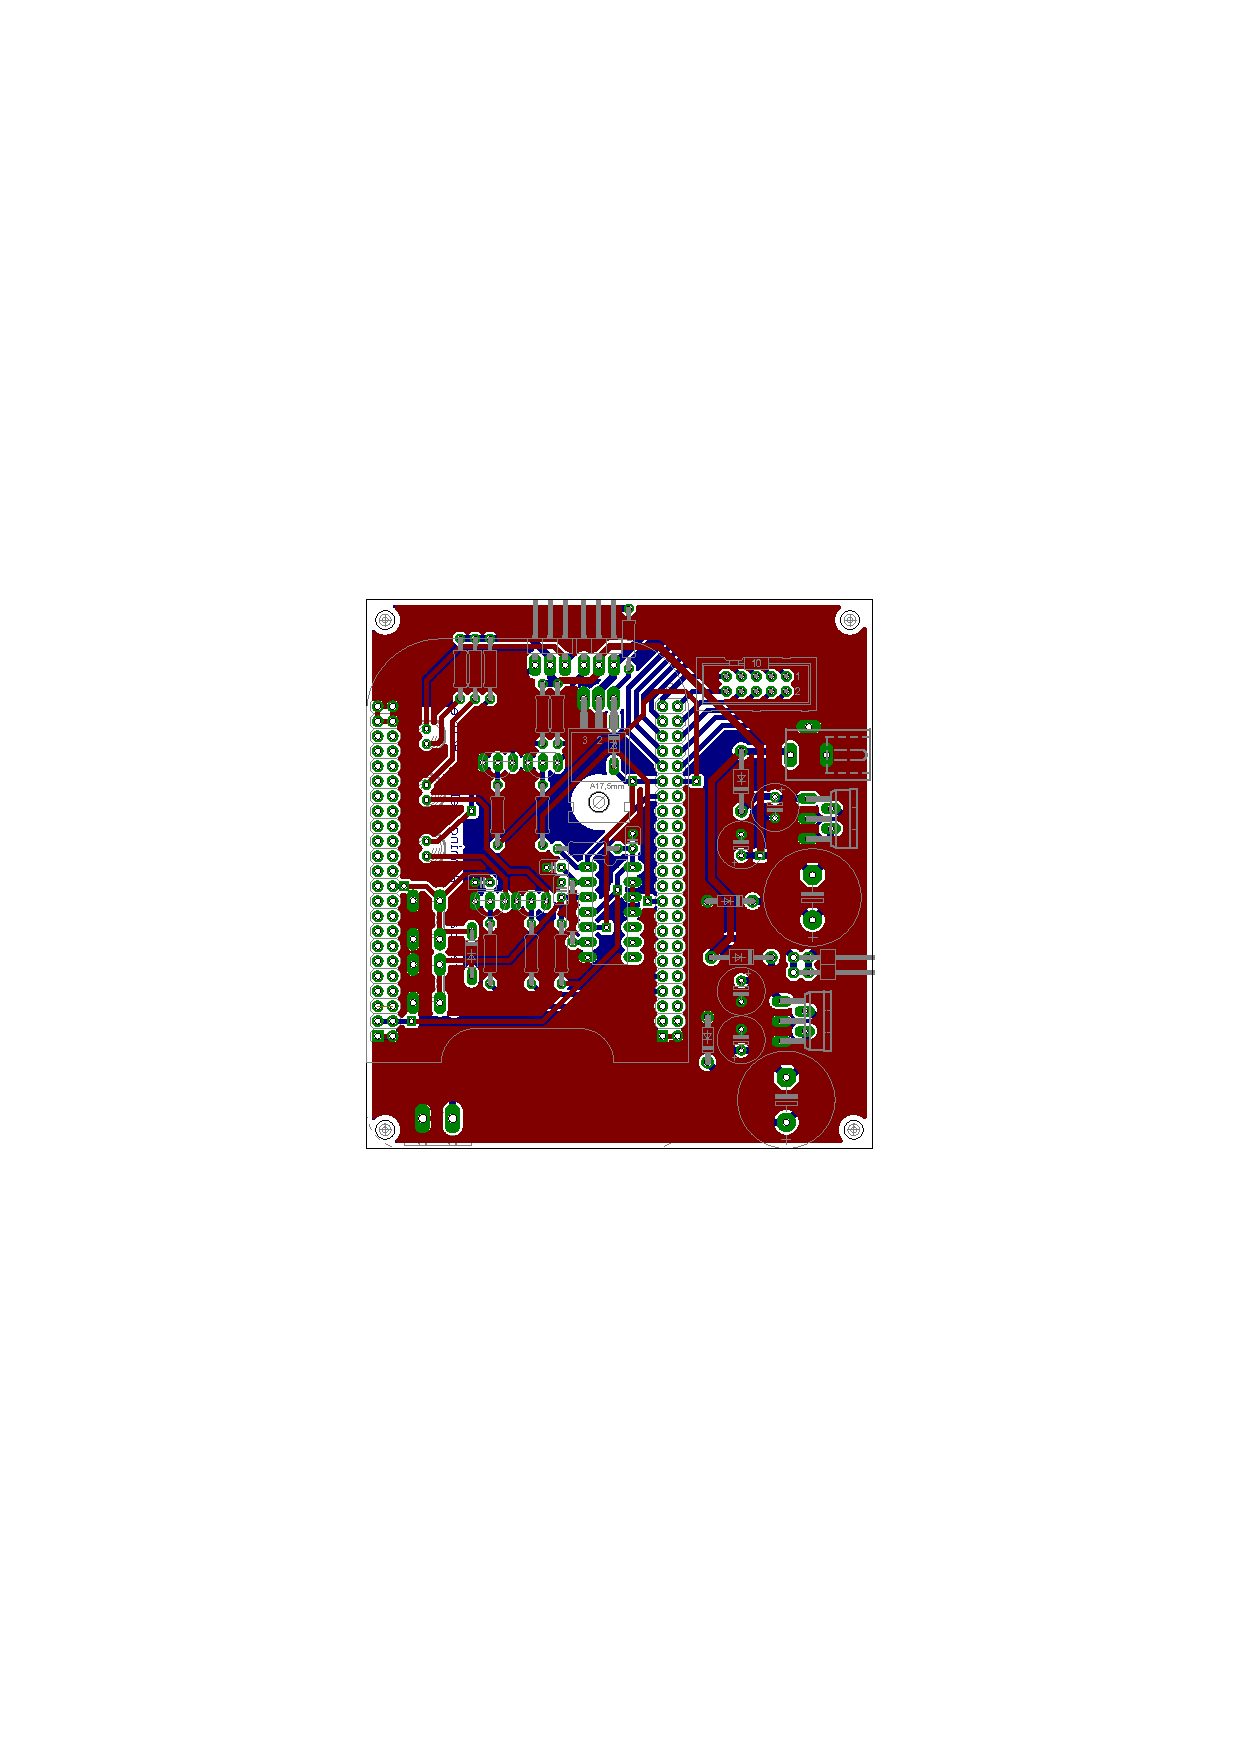
\includegraphics[scale=.75]{appendix/BeagleBoneCape_pcb.pdf}
    \caption{PCB van \emph{BeagleBone cape}}
\end{figure}

    \end{appendices}
\end{document}
